\documentclass[14pt]{article}
\usepackage{grffile}
\usepackage{lastpage}           %-to identify last page
\usepackage{xspace}             %-to force add a space
\usepackage[abspath]{currfile}  %-to find path to this file
\usepackage{xstring,ifthen,xifthen}     %-to manipulate strings
\usepackage{tcolorbox}
\usepackage{changepage}
\usepackage{minted}
\usepackage{enumitem}
\usepackage{fontawesome}

\usepackage{mathtools} % for itemize icon alignment (clap)
\usepackage{etoolbox}
\usepackage{titlesec}
\usepackage{graphicx}           %-to add images
\usepackage{tabularx}
\usepackage{tikz}               %-to create Pfaudler logo
	\usetikzlibrary{shapes.geometric} %-for creating hexagon
\usepackage{pgfplots} 

\tikzset{hex/.style={fill=black,rounded corners=3pt,regular polygon,regular polygon sides=6,minimum size=2.5cm}}

\usepackage[linktoc=all,        %-for clickable links and pdf metadata
            colorlinks=true,
            linkcolor=black,
            urlcolor=black,
            citecolor=black,
            pdfauthor={Kody Quintana},
            pdftitle={PfaudSec readme},
            pdfsubject={},
            pdfkeywords={},
            pdfproducer={},
            pdfcreator={}]{hyperref}

\newcommand{\chref}[3][black]{\href{#2}{\color{#1}{#3}}}%


%-----Font configuration-----%
\usepackage{fontspec}
\setmainfont[
  Path          = ./,
  Ligatures     = TeX,
  UprightFont   = TeX/font/OTF/Pfaudler-Book.otf,
  BoldItalicFont= TeX/font/OTF/Pfaudler-BoldItalic.otf,
  BoldFont      = TeX/font/OTF/Pfaudler-Bold.otf,
  ItalicFont    = TeX/font/OTF/Pfaudler-BookItalic.otf,
  %Scale         = 0.9
]{Pfaudler}
%----------------------------%



%-----Margin formatting-----%
\usepackage[paperwidth=8.5in, paperheight=11in]{geometry}
\geometry{top=0.9in, bottom=0.9in, left=0.9in, right=0.9in}
%---------------------------%



%-----Pfaudler colorscheme-----%
\definecolor{pfblue}{RGB}{52,134,199}
\definecolor{pfgrey}{RGB}{125,125,130}
%------------------------------%

\definecolor{backgrey}{RGB}{248,249,250}

\definecolor{bordergrey}{RGB}{234,236,240}

%--------------Pfaudler logo (invoke with \pflogo)---------------%
%---(Must be contained in one paragraph for use in the header)---%
\newcommand\pflogo{%
\raisebox{-9pt}{%
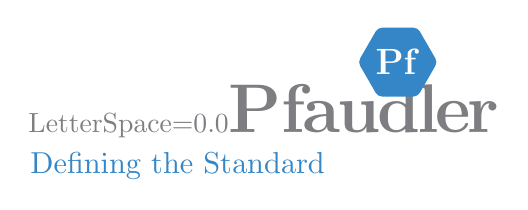
\begin{tikzpicture}
\node [right,scale=1,inner sep=1pt,outer sep=0pt, text=pfblue]
at (0,0) {\fontsize{10.73}{5}\selectfont{%
%
%--Strapline--%
Defining the Standard}};
%
\node [right,scale=1,inner sep=0pt,outer sep=0pt, text=pfgrey]
at (0.01,0.70) {\addfontfeature{LetterSpace=0.0}\fontsize{30}{0}\selectfont{%
%
%--Manually kerned Main text--%
\textbf{%
P{\kern 0.0pt}%
f{\kern-1.0pt}%
a{\kern-1.1pt}%
u{\kern-1.1pt}%
d{\kern-1.1pt}%
l{\kern-1.1pt}%
e{\kern-1.1pt}%
r}%
}};
%
%--Pf hexagon--%
\path (4.70,1.32) node [regular polygon,
		regular polygon sides=6,
		rounded corners=1.5pt,
		inner sep=8.8pt,
		fill = pfblue](hexagon){};
%--Pf hexagon text--%
\node [text=white, scale=1.1] at (4.70,1.32) {\large{\textbf{Pf}}};
\end{tikzpicture}}}
%----------------------------------------------------------------%


\newcommand\pfhexlogo{%

\begin{tikzpicture}
%--Pf hexagon--%
\path (0,0) node [regular polygon,
		scale=0.6,
		regular polygon sides=6,
		rounded corners=1.2pt,
		inner sep=8.8pt,
		fill = black](hexagon){};
%--Pf hexagon text--%
\node [text=white, scale=0.65] at (0,0) {\large{\textbf{Pf}}};
\end{tikzpicture}}

%---------------------------------Header Formatting---------------------------------%
\usepackage{fancyhdr}

%--First page header style--%
\fancypagestyle{style1}{
\fancyhf{}
\fancyhead[L]{\pflogo}
\fancyhead[R]{
P.O. Box 23600, Rochester, NY 14692-3600\\
1000 West Ave. Rochester, NY 14611 USA\\
\begin{tabular}{@{}l r@{}}
Telephone:&\href{tel:5852351000}{1-585-235-1000}\\
Website:&\href{www.pfaudler.com}{www.Pfaudler.com}
\end{tabular}}
\fancyfoot[R]{\large\thepage\xspace of \pageref{LastPage}}
\renewcommand{\footrulewidth}{0.4pt}
\renewcommand{\headrulewidth}{0.4pt}}

%--Embedded documents overlay header--%
\fancypagestyle{style2}{
\fancyhf{}
\fancyhead[R]{\pfhexlogo}
\fancyhead[L]{\textbf{\LARGE PfaudSec DataBook Documentation}}
\fancyfoot[R]{\large\thepage\xspace of \pageref{LastPage}}
\renewcommand{\footrulewidth}{0.4pt}
\renewcommand{\headrulewidth}{0.4pt}}
%-----------------------------------------------------------------------------------%

\newcommand{\pflogoart}{
\raisebox{1cm}{
\hspace{-2.5cm}
\begin{tikzpicture}[scale=1.2,overlay]
\node [hex] (inner) {};
\path (inner.center) node[text=white]{\fontsize{32}{32}\selectfont\textbf{Pf}};
\path (inner.center) ++({360/6*(1-0.5)}:2cm)  node[hex]{} node[text=white]{\Large\textbf{Quality}}; %1
\path (inner.center) ++({360/6*(6-0.5)}:2cm)  node[hex]{} node[text=white]{\normalsize\textbf{Assurance}}; %6
\end{tikzpicture}
}}


\titleformat{\section}
{\normalfont\LARGE\bfseries}{\thesection}{0.5em}{}
\titleformat{\subsection}
{\normalfont\Large\bfseries}{\thesubsection}{0.5em}{}
\titleformat{\subsubsection}
{\normalfont\bfseries}{\thesubsubsection}{0.5em}{}
\titleformat{\paragraph}[runin]
{\normalfont\large\bfseries}{\theparagraph}{0.5em}{}
\titleformat{\subparagraph}[runin]
{\normalfont\large\bfseries}{\thesubparagraph}{0.5em}{}

%-----------Table of Contents Formatting-----------%
%----(compiler must be ran twice to update TOC)----%
\usepackage{titletoc}

%--section toc format--%
\titlecontents{section}
[3em]
{}
{\contentslabel{1em} }
{}
{\titlerule*[0.7pc]{.}\contentspage}

%--subsecion toc format--%
\titlecontents{subsection}
[6em]
{\hangindent1em}
{\contentslabel{1.7em}}
{}
{\titlerule*[0.7pc]{.}\contentspage}

\renewcommand\thesubsubsection{\thesubsection \xspace (\alph{subsubsection})}

\titlecontents{subsubsection}
[7em]
{}
{}%{\contentslabel{3.7em}}
{}
{\titlerule*[0.7pc]{.}\contentspage}

%--Page number formatting--%
\makeatletter
\renewcommand{\contentspage}[1][\thecontentspage]{\hb@xt@\@pnumwidth{#1\hfil}\hspace*{-\@pnumwidth}}
\renewcommand{\@pnumwidth}{3em}
\makeatother

%--------------------------------------------------%

%\setlength{\parskip}{12pt}

%-------------Page embedder-------------%
\usepackage{pdfpages}
%---------------------------------------%


\thispagestyle{style1}
\pagestyle{style2}
\AtBeginDocument{\vspace*{2\baselineskip}}

%file/folder list with fontawesome icons
\setlist[enumerate,1]{label=\bfseries\arabic*)}
\SetLabelAlign{center}{\clap{#1}}
\newcommand{\ifolder}{\item[\faFolderOpen]}
\newcommand{\ifile}{\item[\faFileText]}





%%%%%                                                                                                       %%%%%
%%%%%  ____                   _             _____                                                      _    %%%%%
%%%%% |  _ \                 (_)           |  __ \                                                    | |   %%%%%
%%%%% | |_) |   ___    __ _   _   _ __     | |  | |   ___     ___   _   _   _ __ ___     ___   _ __   | |_  %%%%%
%%%%% |  _ <   / _ \  / _` | | | | '_ \    | |  | |  / _ \   / __| | | | | | '_ ` _ \   / _ \ | '_ \  | __| %%%%%
%%%%% | |_) | |  __/ | (_| | | | | | | |   | |__| | | (_) | | (__  | |_| | | | | | | | |  __/ | | | | | |_  %%%%%
%%%%% |____/   \___|  \__, | |_| |_| |_|   |_____/   \___/   \___|  \__,_| |_| |_| |_|  \___| |_| |_|  \__| %%%%%
%%%%%                  __/ |                                                                                %%%%%
%%%%%                 |___/                                                                                 %%%%%

\begin{document}

\setlength\headheight{20pt}
%\setlength{\footskip}{60pt}
\begin{flushleft}

\fontsize{35}{35}\selectfont\textbf{PfaudSec DataBook\\ Documentation}\\

\normalsize
%\AtBeginEnvironment{quote}{\itshape}

%-----Table of Contents-----%
\setcounter{tocdepth}{2}
\setcounter{secnumdepth}{3}
\startcontents[section]
\begin{center}
\setlength{\parskip}{0.5em}
\printcontents[section]{}{1}{}
\setlength{\parskip}{1em}
\end{center}
%---------------------------%

%use for subsubsection indentation
\newenvironment{subs}
  {\adjustwidth{2em}{0pt}}
  {\endadjustwidth}



\section{About}

PfaudSec (short for Pfaudler Secretary) is a tool for compiling multiple portable document format (PDF) files into a single PDF file.
Additionally, a cover page is generated to include the job information and a table of contents for the included documents.

\section{Dependencies}

This section describes PfaudSec's dependencies, for installation instructions see:
\hyperref[sec:install]{\textit{Installing from source}}.\\[\normalbaselineskip]
PfaudSec is a Python based interface for generating documents with the \LaTeX\xspace typesetting language.
Its GUI is provided by the Qt5 library (via the PyQt5 wrapper).
Document repair and compression is done by Ghostscript.

	\subsection{Python}
PfaudSec is written primarily in Python.
From pythondocs.org:

\begin{quote}
Python is an interpreted, object-oriented, high-level programming language with dynamic semantics. Its high-level built in data structures, combined with dynamic typing and dynamic binding, make it very attractive for Rapid Application Development, as well as for use as a scripting or glue language to connect existing components together. Python's simple, easy to learn syntax emphasizes readability and therefore reduces the cost of program maintenance. Python supports modules and packages, which encourages program modularity and code reuse. The Python interpreter and the extensive standard library are available in source or binary form without charge for all major platforms, and can be freely distributed.\end{quote}

%\newpage
The following Python modules are not part of the standard library and must be installed with pip:

		\begin{subs}
		\subsubsection{PyQt5}
PyQt5 is a Python wrapper for enabling the use of the Qt5 C++ GUI framework with Python.
The GPL version that is utilized by PfaudSec includes the binaries for Qt5, so Qt does not need to be installed separately.

		\subsubsection{PyInstaller}
PyInstaller is a Python module used for packaging the Python source .py files, a Python interpreter, and all Python modules into a single .exe file.

		\subsubsection{QDarkStyle}
QDarkStyle is a dark theme for Qt

		\subsubsection{PyCryptodomex}
Python encryption module (used for distributing commercial font)

		\subsubsection{FontTools}
Python font tools, used to validate decrypted fonts
		\end{subs}

	\subsection{Qt}
The high level GUI framework for PfaudSec is provided by Qt5, however the binaries for Qt are included in the Python module PyQt5 and do not need to be installed separately.
If you would like to make changes to the interface layout file (redirect.ui) Qt should be installed for access to its graphical interface editor QtCreator.

	\subsection{Ghostscript}
Ghostscript is an interpreter for the PostScript language and for PDF files.
PDFs input to PfaudSec are all opened and processed by Ghostscript first to fix any errors and (optionally) add compression.

	\subsection{TexLive}
Texlive is a distribution of the \LaTeX\xspace typesetting language that provides binaries and packages.
PfaudSec utilizes the XeLaTeX engine for compiling the final PDF.

\section{Installing from source}
\label{sec:install}

After downloading the PfaudSec source, follow these steps to prepare the package for use on Windows.

\begin{enumerate}

\item \textbf{Install Python.}

PfaudSec requires Python 3.6 or newer.
Installers are available at
\chref[pfblue]{https://www.python.org/downloads/}{https://www.python.org/downloads/}
After installing Python, ensure that its installation folder and scripts subfolder have been added to your PATH system variable.
If these folders are not correctly added to PATH you will receive the following message: 
``python is not recognized as an internal or external command, operable program or batch file.''

\item \textbf{Install Python modules}

Python modules that are not part of the standard library can be installed with pip, the Python package manager.
Pip is included with Python, if the command is not found ensure that ``.../python3x/scripts'' has been addded to PATH.
Also, if you are installing packages to a system wide Python installation you must run this command in an elevated command prompt.

Open a terminal and enter the following commands:

\begin{tcolorbox}[boxrule=0.5pt, colback=backgrey, colframe=bordergrey, sharpish corners] 
\begin{minted}{bash}

pip install pyqt5

\end{minted}
\end{tcolorbox}

\begin{tcolorbox}[boxrule=0.5pt, colback=backgrey, colframe=bordergrey, sharpish corners] 
\begin{minted}{bash}

pip install pyinstaller

\end{minted}
\end{tcolorbox}

\begin{tcolorbox}[boxrule=0.5pt, colback=backgrey, colframe=bordergrey, sharpish corners] 
\begin{minted}{bash}

pip install qdarkstyle

\end{minted}
\end{tcolorbox}


\begin{tcolorbox}[boxrule=0.5pt, colback=backgrey, colframe=bordergrey, sharpish corners] 
\begin{minted}{bash}

pip install pycryptodomex

\end{minted}
\end{tcolorbox}


\begin{tcolorbox}[boxrule=0.5pt, colback=backgrey, colframe=bordergrey, sharpish corners] 
\begin{minted}{bash}

pip install fonttools

\end{minted}
\end{tcolorbox}

\item \textbf{Package into exe}

Python is an interpreted language so it does not need to be compiled, however packaging the source code with an interpreter can be done for convenience.
This also allows for the program to be run from a network drive without requiring the end user to have Python installed.
To package the program, open a terminal and navigate to the PfaudSec folder then enter:

\begin{tcolorbox}[boxrule=0.5pt, colback=backgrey, colframe=bordergrey, sharpish corners] 
\begin{minted}{bash}

pyinstaller --onefile --windowed --icon=TeX/db_logo.ico main.py

\end{minted}
\end{tcolorbox}

A folder called ``dist'' should now be found in the PfaudSec folder.
Copy the following items from the PfaudSec folder into the dist folder:

\begin{tcolorbox}[boxrule=0.5pt, colback=backgrey, colframe=bordergrey, sharpish corners] 
\begin{itemize}[labelsep = 1.5em, align=center]% leftmargin=0.5in]

\ifolder TeX
\ifile sections\_config.ini

\end{itemize}
\end{tcolorbox}

Next, rename main.exe inside dist to PfaudSec\_DataBook.exe

\item \textbf{Install TexLive}

An installer for TexLive is available at:
\chref[pfblue]
{https://www.tug.org/texlive/acquire-netinstall.html}
{https://www.tug.org/texlive/acquire-netinstall.html}
It is recommended to download the
``install-tl.zip'' and not the ``install-tl-windows.exe''
as running the bat file found inside the zip will give more verbose output should the installer fail.

After extracting the contents of ``install-tl.zip'', run ``install-tl-advanced.bat''.
Toggle portable setup to yes, and select ``.../PfaudSec/dist/texlive'' as the installation folder.
The installation will take a while, the full distribution of TexLive is several gigabytes in size.

\item \textbf{Install Ghostscript}

A portable version of Ghostscript has been made available at
\chref[pfblue]
{https://portableapps.com/apps/utilities/ghostscript_portable}
{https://portableapps.com/apps/utilities/ghostscript\_portable}
Run the installer and choose ``.../PfaudSec/dist/Ghostscript/'' as the installation directory.

\item \textbf{Copy to network drive}

PfaudSec is designed to be portable and can be run from a network drive.
Rename the dist folder to PfaudSec\_DataBook and copy it to wherever you would like to run it from.
A user procedure can be added to the folder with the name ``user\_procedure.pdf'' this PDF can be opened with the help > user procedure button in PfaudSec.

%\newpage
The final folder should contain the following:

\begin{tcolorbox}[boxrule=0.5pt, colback=backgrey, colframe=bordergrey, sharpish corners] 

\begin{itemize}[labelsep = 1.5em, align=center]

\ifolder Ghostscript
\ifolder TeX
\ifolder texlive
\ifile PfaudSec\_DataBook.exe
\ifile sections\_config.ini
\ifile user\_procedure.pdf

\end{itemize}
\end{tcolorbox}

If PfaudSec has already been installed and you are only upgrading, only the exe file should be copied.

Due to the license of the font used by Pfaudler, the included font has been encrypted, the password will have been provided to you.
PfaudSec will prompt you for this password only the first time it is run.


\end{enumerate}

\section{Usage}
\setlength{\parindent}{0.2in}
PfaudSec DataBook scans a user defined folder for PDF files matching the ``basename x.xx.pdf''
format, where basename can be any word with no spaces. (usually MO number) followed by a space, then x.xx which is a numerical shorthand,
These numerical shorthands are defined in sections\_config.ini.

This shorthand naming scheme is used for two reasons. First, so that only PDF files renamed to this format are included while omitting all others, and second so that documents from a scanner are easier to name.
(where often only a physical numpad is available and not a full keyboard).
Included documents are placed in a cover page table of contents based on which section they are defined under in sections\_config.ini.
Entries in sections\_config.ini must be unique.

\begin{tcolorbox}[
coltitle=black, title=\centering Example sections\_config.ini,
boxrule=0.5pt, colback=backgrey, colframe=bordergrey, sharpish corners] 
\begin{minted}{bash}

[Section One name]

1.1 = Document full name
1.2 = Other document full name

[Another section name]

2.1 = Another document

\end{minted}
\end{tcolorbox}

\noindent Job information is entered manually by the user. The program will not render a PDF until all job info fields have been filled in and a folder to pull PDF documents from has been selected.

A ``loose file'' option also exists for inserting pages from a Brazil databook or other source where all PDF files from the specified folder are included and named as they are found.
After the document has completed being compiled, it will open and should be inspected for any errors.
\setlength{\parindent}{0in}

\section{Modifying cover page}

To make changes to the cover page, open TeX/databook.tex with any text editor.
Exercise caution when modifying this file as its contents contain some of the core functionality of PfaudSec DataBook.
A guide to \LaTeX\xspace syntax is available at 
\chref[pfblue]
{https://en.wikibooks.org/wiki/LaTeX/Basics}
{https://en.wikibooks.org/wiki/LaTeX/Basics}

%\newpage
\section{License}

Due to the licenses of PyQt5 and Ghostscript, PfaudSec must be also released under a compatible license.
In this case the GNU Affero General Public License (AGPL).
A full copy of the license can be found with the source code.
While not legal advice, the AGPL can be summarized as follows:\\[\normalbaselineskip]

\def\tabularxcolumn#1{m{#1}}% verticle centering
\newcolumntype{Y}{>{\centering\arraybackslash}X}
\begin{tabularx}{\textwidth}{YYY}

\begin{tcolorbox}[
	equal height group=license, coltitle=black, title=\centering Must,
	boxrule=0.5pt, colback=backgrey, colframe=bordergrey, sharpish corners] 
\begin{itemize}[leftmargin=*]

\raggedright
\item Include Copyright
\item Include License
\item State Changes
\item Disclose Source
\item Include Install Instructions 

\end{itemize}
\end{tcolorbox}

&

\begin{tcolorbox}[
	equal height group=license, coltitle=black, title=\centering Can,
	boxrule=0.5pt, colback=backgrey, colframe=bordergrey, sharpish corners] 
\begin{itemize}[leftmargin=*]

\raggedright
\item Commercial Use
\item Modify
\item Distribute
\item Place Warranty 

\end{itemize}
\end{tcolorbox}

&

\begin{tcolorbox}[
	equal height group=license, coltitle=black, title=\centering Cannot,
	boxrule=0.5pt, colback=backgrey, colframe=bordergrey, sharpish corners] 
\begin{itemize}[leftmargin=*]

\raggedright
\item Sublicense
\item Hold Liable 

\end{itemize}
\end{tcolorbox}

\end{tabularx}

\end{flushleft}
\end{document}
